%% This is an example first chapter.  You should put chapter/appendix that you
%% write into a separate file, and add a line \include{yourfilename} to
%% main.tex, where `yourfilename.tex' is the name of the chapter/appendix file.
%% You can process specific files by typing their names in at the 
%% \files=
%% prompt when you run the file main.tex through LaTeX.
\chapter{Technology research}

This chapter aims to synthesize the research carried on the main knowledge areas involved in the development of this project. It pretends to give an overview of the technologies and paradigms considered to support the design decisions the project is based upon. This includes the main areas of concern: Public Interface, Database, Real time, Web Technologies, Event logging.

\begin{figure}[h]
	\centering
	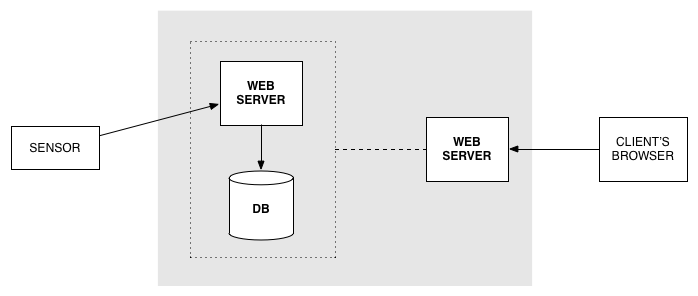
\includegraphics[width=\textwidth]{architecture_analysis}
	\caption{High-level required components}
	\label{fig:arch_analysis}
\end{figure}

\section{Public Interface}

\subsection{Client devices}

In recent years, there has been a steady reduction in costs of hardware devices. Particularly, some microcontrollers have reached prices under 10\$ such as ATmega168, which is the one used by Arduino. Based on a simple microcontroller board and its own development environment, Arduino can be used to develop a vast variety of interactive objects. Its CPU speeds ranging from 8 to 84 Mhz, USB and UART ports, many digital and analog I/O and Flash memory, make it a powerful physical computing device. Even though there are many other affordable microcontroller platforms, Arduino stands out for its easy-to-use programming environment and cross-platform software. It is specially worth mentioning, however, that it is an open-source physical computing platform. Both its software and the plans of its modules are published under open source licenses.

On the other hand, the decrease in the price of processors for mobile devices, with excellent multimedia capabilities led to the foundation of the Raspberry Pi Foundation and the public release of the first Raspberry Pi in 2012. It consists of a single-board computer aimed at teaching computer science basics. Unlike Arduino, it is shipped with 700 MHz ARM processors and as any other computer, it comes with GPU, video and audio outputs and SD storage, but only its Model B has 100 Mbits Ethernet connection. Although it supports some Linux kernel-based operating systems like Debian GNU/Linux and Arch Linux ARM, it is recommended to run Raspbian, a Debian-based free operating system optimized for the Raspberry Pi hardware. These general purpose features and its credit-card size make it a capable computer which can be used in a wide range of scenarios replacing regular desktop PCs.

Both devices have different aims and capabilities. Arduino is a easy-to-use lower-level physical computing platform, whereas Raspberry Pi beats general purpose PCs in terms of cost and size. Nonetheless, it is not unusual to combine their features attaching them together as a single device, which \cite{Arduberry} attempts. While Arduino brings I/O capabilities Raspberry Pi lacks, the latter provides computing power.

These features have contributed to their popularity among people involved in technology as well as computing aficionados. They have attracted great interest in the Internet of Things (IoT) community and have had direct impact on its recent growth. Some project are heavily inspired by Arduino extensibility such as \cite{Thinking-Things}, whilst others build their products based on customized Arduino boards.

This is the case of Smart Citizen a whole platform aimed at generating participatory processes of people in cities thus, creating more effective and optimized relationships between services, technology and communities in the urban environment. The core of the platform is the called Smart Citizen Kit, a hardware device shipped with air, temperature, light, sound and humidity sensors plus a Wi-Fi module to serve as ambient sensor. They started up with Arduino shields to develop a prototype, until eventually coming up with their own specific-purpose arduino-compatible data-processing board.

\subsection{Interoperability}

Interoperability is the software quality of enabling a system to interact with other systems without the need to write or maintain custom logic. This is often achieved using the same protocols, exchange or file formats, or by means of standardization.

Interoperability has a great impact on several fields such as financial or medical industries where inadequate implementations may lead to important economic costs. It also crucial in science since the outcomes of a research must be operable for others in order to progress towards a common goal. This also applies in the context of this project since the data obtained by the sensors and its underlying infrastructure may be used in other research projects of CREAF. Not less important is the role this project plays within CREAF's efforts towards the Sensor Web \cite{SWE} as standardization group of the Open Geospatial Consortium (OGC). Therefore, interoperability is a main concern for REDCH.

The OGC's Observations \& Measurements (O\&M) \cite{OM} is the standard data model for storing and publishing sensor data. Based on the Geography Markup Language (GML) OGC standard, it models the relationship between observation events, the spatial objects under observation, the measured properties and measurement procedure and the captured data resulting from the observations. O\&M is one of the open standards developed in the Sensor Web Enablement (SWE) initiative of the OGC.

While O\&M provides a system-independent way of sensor data exchange, the Sensor Observation Service (SOS), another SWE standard, defines a Web service interface for sensor data. This standard allows querying observations and sensor metadata, registering and removing sensors, as well as inserting new sensor observations. Furthermore, it defines KVP and SOAP bindings so as to be binding-independent. However OGC does not provide an implementation but a service interface.

There are currently some open-source implementations of the SOS. The Earth Science Institute of the University of Applied Sciences of the South Switzerland set up istSOS \cite{istSOS} in 2009. A SOS implementation entirely written in Python that includes a RESTful API and a graphical user interface for easing the administration of the service.

52$\textdegree$North is a network of partners from research, such as the University of Münster and the Technische Universität Dresden, industry, such ESRI Inc. and public administrations such as the IT department of the German Federal Ministry of Transport, Building and Urban Development. It is aimed at bringing innovation in the field of Geoinformatics. 52ºNorth SOS \cite{52north-SOS} is the leading implementation of the Sensor Observation Service. The latest version 4.0, recently released as of this writing, comes with full support of the SOS 2.0 specification. In addition, 52ºNorth has developed the SOS RESTful Extension. A SOS 4.0 Add-on that provides a REST binding beyond the standard KVP and SOAP defined by the OGC.

\section{Database}

The way the data is handled and stored is a key point of the project. Therefore, it is crucial to choose the Database management system (DBMS) that best fits the features of the underlying data set. It must implement some sort of geographic support as every observation implicitly belongs to a particular geolocation.

Databases allow to persist a representation of the real-world objects and their relations in a structured fashion. Furthermore, they also allow to integration the data of different applications thus, avoiding data duplication. 

\subsection{Relational Databases and NoSQL}

Databases may be classified in three general models: hierarchical, network, relational and NoSQL. Relational databases have gain a lot of popularity since their appearance in the late 1970s, becoming the de facto choice regarding data management in IT systems. On the ohter hand, NoSQL systems is a field that is still evolving very fast since its birth in the 2000s.

\paragraph{Relational DBMSs}

The relational model is based on set theory and predicate logic. Relational databases implement an approximation of that mathematical model using a table-based format. The data is structured in tables that represent relations, where the information of a particular entity is represented by a row and the set of fixed attributes of such entity correspond to the columns.

Databases, however, need DBMSs in order to be functional. A DBMS is a software specially designed to allow the creation, querying, update, and management of databases. It is a layer above the OS that abstracts the applications from the database. Hence, applications deal with databases through the DBMS, as they do with files through the OS.

Relational DBMSs essentially provide efficient, reliable, convenient, and safe multi-user storage of and access to massive amounts of persistent data. They guarantee consistency by means of robust concurrency models and ACID (Atomicity, Consistency, Isolation, Durability) transactions. Due to decades of development and research relational database systems are relied upon by mission-critical applications that demand strict consistency.

The most popular open-source relational DBMSs are MySQL and PostgreSQL, both with spatial extensions. PostGIS, however, is the most mature solution. It is a PostgreSQL extension that adds support for location awareness allowing to query by geographic location. In addition, PostGIS supports geographic coordinates. As a consequence of PostGIS' rich feature list PostgreSQL is the standard choice for Geographic Information Systems (GIS).

However, not every data management or analysis problem is best solved exclusively using a traditional DBMS. There are some problems that are more suitable for other type of systems \cite{NoSQL-use-cases}.

\paragraph{NoSQL Systems}

NoSQL Systems, which name stands for \textit{Not Only SQL}, differ from traditional relational systems in that they tend to provide a flexible schema rather than a rigid structure, they are quicker or cheaper to set up, they are geared towards massive scalability and they use relaxed consistency in order to provide higher performance and higher availability.

Their downsides are that there is no declarative query language thus, more programming is involved in manipulating the data. Furthermore, because of the relaxed consistency models, their better performance comes at the expense of fewer guarantees about the consistency of the data. Eventually consistent systems are often classified as providing BASE (Basically Available, Soft state, Eventual consistency) properties in contrast to traditional ACID-compliant relational systems.

One of the main goals of NoSQL systems is to enhance horizontal scalability. As the CAP theorem states \cite{CAP-theorem}\cite{CAP:online}, this can only be achieved by relaxing either its consistency or its availability so partition tolerance may be guaranteed. There is no consensus among NoSQL vendors over which pair to choose. Some opt for consistency against availability, while others focus on availability over consistency \cite{CAP-NoSQL}. Nonetheless, there are few that pick both properties and consequently provide scalability through replication rather than partitioning.

The number of different kinds of NoSQL systems may be generalized in four main categories: MapReduce framework, Key-value stores, Graph database systems and Document stores. MapReduce framework are typically used for applications that process large amounts of data to do complex analysis, whereas Key-value stores tend to perform a lot of small operations on very small parts of the data. On the other hand, Graph database systems are designed for storing and operating over very large graphs.

\paragraph{Document stores}

Document stores are very similar to Key-value stores except that the values are a document. Hence, the data model is based on ${<key, document>}$ pairs where the document is a known type of structure that can contain semistructured formats such as JSON or XML. The basic operations, like key-value stores, allow to fetch, update, delete and insert a document based on a given key. Additionally, they also implement a fetch operation based on document contents which is a very implementation-specific feature since there is no standard query language. Few examples of document stores are CouchDB, MongoDB and Amazon's SimpleDB, among many others.  

In addition, MongoDB, CouchDB and SimpleGEO support geospatial indexing allowing to query for location-based data. Although not as accurate as PostGIS, these NoSQL systems may fit in some use cases where performance and scalability are a major issue.

\section{Real Time in Distributed Systems}

As defined in \cite{distributed-systems-book} a distributed system is \textit{a collection of independent computers that appears to its users as a single coherent system}. This involves some sort of collaboration between the autonomous components (i.e., computers). Although discussing the advantages and disadvantages is not the topic of this writing, the main benefits of distributed architectures over centralized systems are the greater scalability, improved resilience and higher availability. To do so, distributed systems decouple a single application in a number of components that handle the diverse functionalities of the whole system. This allows to horizontally scale the components in an independent way and make them fail-tolerant. However, this impose other problems. The components need to share state and communicate. Moreover, handling failure is often a complex task.

The challenge a real time in a distributed environment entails is essentially the management of the system's state. 

- why state a problem in DS
- pull vs push

\subsection{Asynchronous Messaging Queue}
RabbitMQ
ZeroMQ

- impact on client
- Async app server. Reactor pattern.

\subsection{Tuple Space}
redis

\section{Web Technologies}

Since the Sir Tim Berners-Lee's first draft of the World Wide Web back in 1989 and his first proposal for the HyperText Markup Language (HTML) \cite{HTMLtags} in 1991 the WWW has experienced a tremendous evolution. Since then, HTML has gone through many revisions. The World Wide Web Consortium (W3C) published many iterations of the standard until the specification HTML 4.01 in 1999. It was not until 2004 that HTML was proposed to be extended so as to allow the creation of web applications. This led to the publication of the First Public Working Draft of the HTML5 specification in 2008. Although parts of HTML5 have been implemented in browsers it hadn't been until 2012 that W3C designated HTML5 as a Candidate Recommendation and it is planned to be released as a stable Recommendation by the end of 2014.

HTML5	
	- what is it
	- who
	- future
	- APIs: Canvas, SVG, ... particularly the ones involved in Redch

Browser vendors
	- dramatic improvement of JS engines
	- prefixed CSS properties and non-standarized prefixed APIs

	- Towards application platform
		- Firefox OS, Node.js (JS in the backend), Win8 JS apps, 
		- rich applications GDocs, Chrome book

JS Libraries
	- to solve cross-browser issues/compatibility, old browsers. jQuery
	- D3, widely used. Standard for data visualization. As being the 5th most starred repository in github, more than rails or angular.js, shows.
	- Chart.js

JS apps -> Redch web application 
	- Ajax
	- problem of JS apps -> old browsers. Autoupdate
	- Backbone, underscore -> Angular.js, Ember
	- full ecosystem of MVC components, templates systems, etc.

\subsection{Server Sent Events}
specification over standard HTTP. RFC

\subsection{Web Sockets}
buzzword, trend, full duplex
Too often misunderstood, lower level protocol than HTTP, whole new protocol

\section{Event Logging}
Need to get insight of the system functioning. Misbehaviour. Analysis tool.
